\documentclass[referee]{aa}
\usepackage{graphicx}
\usepackage{txfonts}

\begin{document}

\title{Efficient Hamiltonian splitting of multiscale $N$-body systems}

\author{
J\"urgen J\"anes\inst{1,2}\and
Inti Pelupessy\inst{3}\thanks{
Corresponding author. Tel.: +31 715278424; fax: +31 715275743.\\
E-mail address: pelupes@strw.leidenuniv.nl (F.I. Pelupessy).}\and
Simon Portegies Zwart\inst{3}
}

\institute{
The Gurdon Institute and Department of Genetics, University of Cambridge, Cambridge CB3 0DH, United Kingdom\and
Faculty of Science, University of Amsterdam, P.O. Box 94216, 1090 GE, Amsterdam, The Netherlands\and
Leiden Observatory, Leiden University, P.O. Box 9513, 2300 RA, Leiden, The Netherlands
}

\date{Received XX; accepted YY}

\abstract{Here be dragons.}

\maketitle

\section{Introduction}
A typical schema for direct integration of a gravitational $N$-body
system consists of advancing the state of the system by small discrete
time steps while in some way approximating the gravitational forces
acting between every pair of particles. This calculation is a computationally
intensive, as the number of forces that need to be considered scales
with $N^{2}$, and we need to take small steps to obtain an accurate
solution.

For systems with a large range of time scales for different interactions
--- as is often the case with astrophysical initial conditions ---
the calculation can be made more efficient by exploiting the ``sparseness''
of the problem. Figurativelly, the interaction between two stars in
a close binary with an orbital period of a few days at the centre
of a Plummer sphere can be evaluated at signifiantly higher precision
compared to a slowly moving star at the edge of a Plummer sphere.

A widely used approach to taking advantage of this sparseness is a block time step scheme where each particle is assigned a time step in a power of two hierarchy. Typically, in these kinds of block time step schemes, the total force acting on a particle in a fast bin is calculated by extrapolating the positions of particles in slower bins.(Aarseth, Konstantinidis, etc...) This extrapolation is known to lead to loss of conservation of momentum.(Cite?)

We have previously derived momentum-conserving integrators for arbitrary $N$-body systems via recursivelly splitting the Hamiltonian of the system.\cite{Pelupessy:2012if} This is achieved by considering forces between particles in different bins in ``pairs''.

In this work, we introduce a new method for splitting the Hamiltonian of the system. Specifically, we partition the system using connected components of the graph generated by the time step criterion. Numerical experiments show that this decomposition leads to performance gains even for a straightforward Plummer sphere, where the presence of isolated subsystems is not immediatelly obvious. For astrophysically realistic systems explicitly chosen for their multi-scale behaviour, the performance gains increase considerably.

Implementations of the splitting methods are incorporated in the HUAYNO integrator, which is available as a part of the AMUSE framework.\cite{Pelupessy:2013tv}

\section{Method}

\subsection{The optimal Hamiltonian splitting problem}

The Hamiltonian for a system of $N$ particles $i=1\ldots N$ under
gravitational interaction can be represented as a sum of momentum
terms $T_{i}$ and potential terms $V_{ij}$:

\begin{eqnarray*}
H(\mathbf{p}_{i},\mathbf{q}_{i}) & = & T+V=\underset{i=1}{\overset{N}{\sum}}T_{i}+\underset{\substack{i,j=1\\
i<j
}
}{\overset{N}{\sum}}V_{ij}\\
T_{i} & = & \frac{\left|\mathbf{p}_{i}\right|^{2}}{2m_{i}}\\
V_{ij} & = & -G\frac{m_{i}m_{j}}{\sqrt{q_{ij}^{2}+\varepsilon^{2}}}
\end{eqnarray*}
where $m_{i}$ is the mass, $\mathbf{q}_{i}$ is the position and
$\mathbf{p}_{i}$ is the momentum of the$i$-th particle of the system.

Let the Hamiltonian $H$ of the system be representable as a sum of
two sub-Hamiltonians, $H=A+B$. We can approximate the time evolution
under $H$ with a sequence of time evolution steps under the sub-Hamiltonians
$A$ and $B$. A straightforward successive application of the time
evolution under $A$ followed by the time evolution under $B$ gives
a first-order approximation of the full time evolution under $A+B$,
while a second-order accurate approximation can be obtained with one
additional operator evaluation \cite[Sec 12.4]{SSC94}.
\begin{equation}
\operatorname{E}_{h,A+B}=\operatorname{E}_{h/2,A}\operatorname{E}_{h,B}\operatorname{E}_{h/2,A}+\operatorname{O}\left(h^{2}\right)\label{eq:second-order-kick}
\end{equation}
Here, the sub-Hamiltonian $A$ is evolved in two steps of $h/2$ and
the sub-Hamiltonian $B$ is evolved in a single step $h$. We can
take advantage of this property of the splitting formula by dividing
terms associated with fast interactions into $A$ and terms associated
with slow interactions into $B$. We can proceed by applying this
splitting procedure to different sub-Hamiltonians multiple times,
thereby constructing an integrator that evaluates parts of the Hamiltonian
at $h$, $h/2$, $h/4$ etc, similarly to the power of two hierarchy
used in block time step schemes.

Both Hamiltonians consisting of a single momentum term and Hamiltonians
consisting of a single potential term have an analytical solution.
For a single momentum term of the $i$-th particle

\[
H_{i}(\mathbf{p}_{i},\mathbf{q}_{i})=T_{i}=\frac{\left\langle \mathbf{p}_{i},\mathbf{p}_{i}\right\rangle }{2m_{i}}
\]
the solution consists updating the position of the $i$-th particle
under the assumption of constant velocity for a time period of $h$
(all positions except the position of the $i$-th particle and the
momenta of all particles remain unchanged). 

\[
\mathbf{q}_{i}(t+h)=\mathbf{q}_{i}(t)+h\mathbf{v}_{i}(h)
\]
We call the time evolution operator for the momentum term of the $i$-th
particle the drift operator and write $D_{h,T_{i}}$.

For a single potential term between particles $i$ and $j$

\[
H_{ij}(\mathbf{p}_{i},\mathbf{q}_{i})=V_{ij}=-G\frac{m_{i}m_{j}}{\sqrt{q_{ij}^{2}+\varepsilon^{2}}}
\]
the solution consists of updating the momenta of the $i$-th and $j$-th
particles under the assumption of constant force for a time period
of $h$ (all momenta except the momenta of the $i$-th and $j$-th
particles and the positions of all particles remain unchanged). 
\begin{eqnarray*}
\mathbf{p}_{i}(t+h) & = & \mathbf{p}_{i}(t)+h\mathbf{F}_{ij}(t)\\
\mathbf{p}_{j}(t+h) & = & \mathbf{p}_{j}(t)+h\mathbf{F}_{ji}(t)
\end{eqnarray*}
 We call the time evolution operator for the potential term between
the $i$-th and $j$-th particles the kick operator and write $K_{h,V_{ij}}$.

Now, let $\tau(i)$ be a function giving the minimal time step necessary
for evaluating the momentum term $T_{i}$, and $\tau(i,j)$ be a function
giving the minimal time step necessary to evaluate a potential term
$V_{ij}$.%
\footnote{The discussion here is largely unaffected by the exact form of $\tau(i)$
and $\tau(i,j)$; we use the explicit but approximate criterion introduced
in \cite{Pelupessy:2012if} in our implementation.%
} A splitting method for evolving the entire system $H$ while exploiting
the sparseness of the problem to the maximum extent would need to
have the following two properties.
\begin{enumerate}
\item Each kick $K_{h,V_{ij}}$ should be evolved such that $h\leq\tau(i,j)$,
with $h$ being ``as large as possible'' (ideally $2h>\tau(i,j)$).
\item Each drift $D_{h,T_{i}}$ should be evolved such that $h\leq\tau(i)$,
with $h$ being ``as large as possible'' (ideally $2h>\tau(i)$).
\end{enumerate}
We explicitly write the phrase ``as large as possible'' in quotes
to emphasize that finding a decomposition of the system into individual
kicks and drifts also costs computational resources. In other words,
a fast splitting algorithm that evaluates some kicks at smaller time
steps than strictly given by the conditions stated above may be more
desirable from a slow but exact splitting. On the other hand, the
requirement that every term is evaluated at a time step that is at
least $\tau(i,j)$ for kicks and at least $\tau(i)$ for drifts is
strict and must be guaranteed by any splitting algorithm.

In \cite{Pelupessy:2012if}, we introduced the HOLD method of splitting
the Hamiltonian that, given a pivot time step $h$, divides particles
$i=1\ldots N$ into a slow set $S$ and a fast set $F$, essentially
like the partitioning step of the quicksort sorting algorithm.
\begin{eqnarray*}
S & = & \left\{ i\in1\ldots N:\,\tau(i)\geq h\right\} \\
F & = & \left\{ i\in1\ldots N:\,\tau(i)<h\right\} 
\end{eqnarray*}
Based on these two sets $S$ and $F$, we proceed by splitting the
Hamiltonian of the system into the following parts.

\begin{eqnarray}
H & = & H_{S}+H_{F}+V_{SF}\label{eq:SF-splitting-rule}
\end{eqnarray}
$H_{S}$ contains all drifts of particles inside $S$ and all kicks
where both particles are inside $S$. The $H_{F}$ term is defined
in exactly the same way by particles inside $F$. The mixed term $V_{SF}$
contains all kicks where one particle is in $S$ and the other is
in $F$.

Consider now the previously outlined criteria for a splitting method.
By definition of $S$, all terms inside $H_{S}$ can be evolved at
$h$ without violating the time step criteria. By definition of $F$,
all drifts and some kicks in $H_{F}$ should be evolved at a time
step smaller than $h$.

All kicks in $V_{SF}$ can be evolved at $h$. For proof, assume two
particles with indices $s$ and $f$ such that $s\in S$, $f\in F$
and $V_{sf}<h$. Then $\tau(s)<h$ meaning that $s\in F$ which contradicts
$s\in S$.

We now split the evolution of the system into a part that fulfills
the time step criteria and a part that does not fulfill the time step
criteria by applying the second-order Hamiltonian splitting rule.

\begin{eqnarray}
\operatorname{E}_{h,H} & = & \operatorname{E}_{h,H\rightarrow H_{S}+H_{F}+V_{SF}}\\
 & \approx & \operatorname{E}_{h/2,H_{F}}\,\operatorname{E}_{h,H_{S}+V_{SF}}\operatorname{E}_{h/2,H_{F}}
\end{eqnarray}
As discussed previously, all the terms in $H_{S}=T_{S}+V_{S}$ and
$V_{SF}$ can be evolved at the time step $h$. We further decompose
this part into a second order composition of explicit drifts and kicks.

\begin{eqnarray}
\operatorname{E}_{h,H_{S}+V_{SF}} & = & \operatorname{E}_{h,T_{S}+V_{S}+V_{SF}}\\
 & \approx & \operatorname{D}_{h/2,T_{S}}\operatorname{K}_{h,V_{S}+V_{SF}}\operatorname{D}_{h/2,T_{S}}
\end{eqnarray}
Now consider the term $H_{F}$ which is an isolated Hamiltonian consisting
of all drifts in $F$ and all kicks between particles in $F$. We
know that some of the terms in $H_{F}$ cannot be evolved at $h$.
We solve the problem by applying the same splitting procedure described
above with a smaller time step $h/2$, making the definition of the
evolve operator for the SF split recursive. Since the threshold time
step $h$ gets smaller with each application, the recursion will terminate
when all of the particles left in the Hamiltonian are put into the
$S$ set.

The HOLD method always evolves kicks between fast particles at a fast(=small)
time step. This may result in a huge inefficiency if there are several
fast subsystems where interactions between these subsystems could
be evolved at a slow(=large) time step. In particular, consider the
following examples.
\begin{itemize}
\item In a system of several globular clusters, each individual globular
cluster is a subsystem.
\item In a globular cluster with planets around some of the stars, each
star with the orbiting planets is a subsystem.
\item In a single globular cluster, each close encounter between two or
more particles is a subsystem.
\end{itemize}
As an extreme example, consider a Plummer sphere where each star is
in a binary system. In this case, every star has a close binary interaction
that needs to be evaluated at a fast time step. However, the HOLD
integrator will in this case integrate all interactions, including
long-range interactions between stars in different binaries at a fast
time step (determined by one of the binary interactions). This is
essentially equivalent to evolving the entire system with a shared
global time step. For an efficient splitting method, we would want
to evaluate these long-range interactions at a time step closer to
(with the exception of interactions involved in binary-binary close
encounters). 


\subsection{Connected Components splitting}

Consider a system of $N$ particles and a threshold time step $h$.
We construct a split from the connected components\cite[Sec B.4]{Cormen:2001uw}
of the undirected (and unweighted) graph generated by the time step
criteria $\tau(i,j)$. Specifically, the particles of the system form
the vertices of the graph, and there is a edge between particles $i$
and $j$ if their interaction cannot be evaluated at the current threshold
time step $h$: 
\[
\tau(i,j)<h
\]


\begin{figure}
%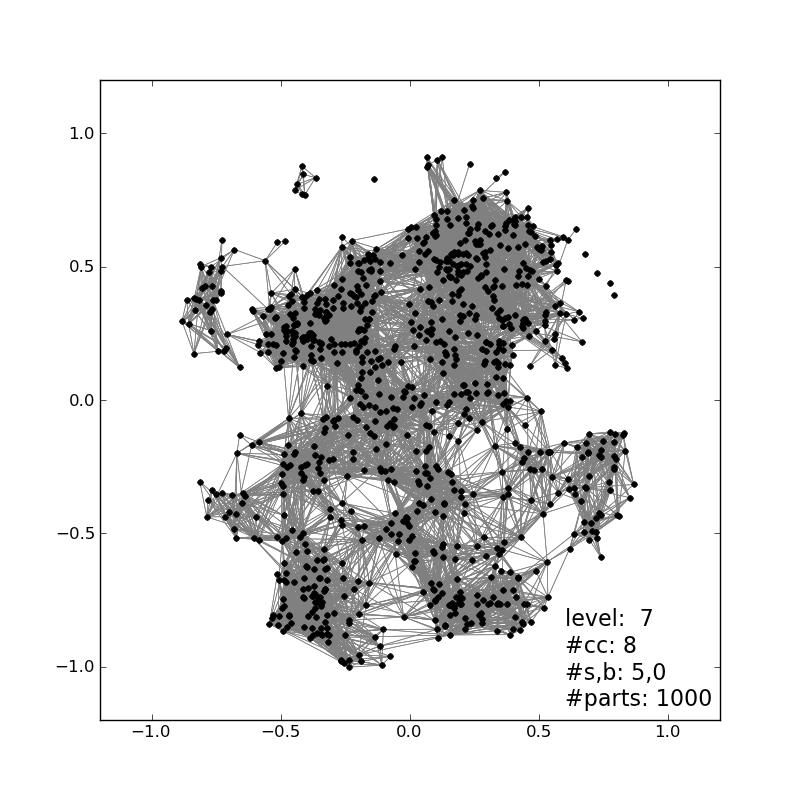
\includegraphics[scale=0.3,bb = 0 0 200 100, draft, type=eps]{/Users/jj374/castle/5hs-paper2/cc_paper-svn/1_cc_illustration/cc-2.3-007.png}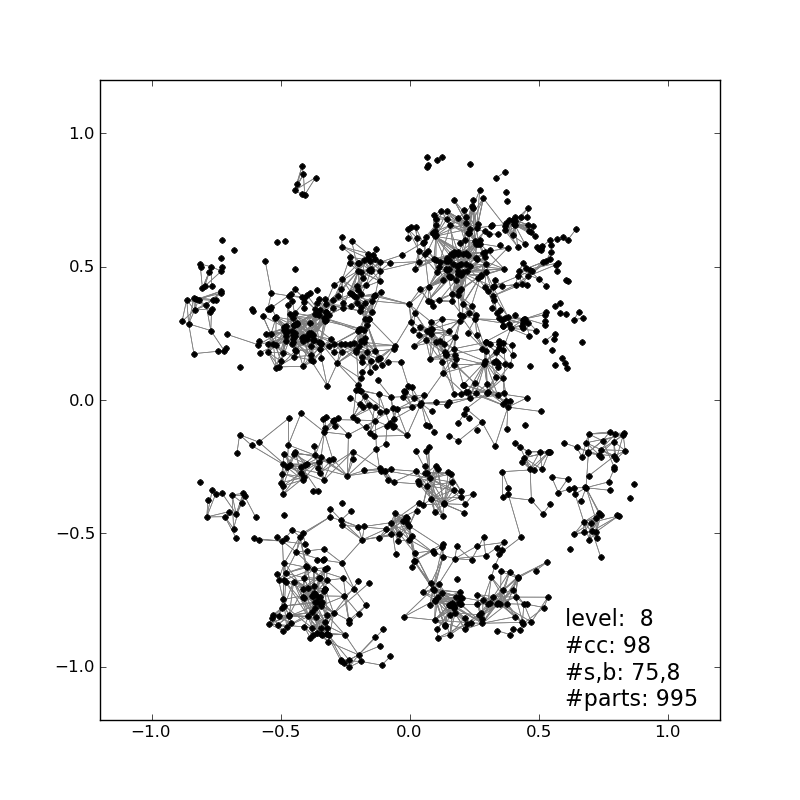
\includegraphics[scale=0.3,bb = 0 0 200 100, draft, type=eps]{/Users/jj374/castle/5hs-paper2/cc_paper-svn/1_cc_illustration/cc-2.3-008.png}

%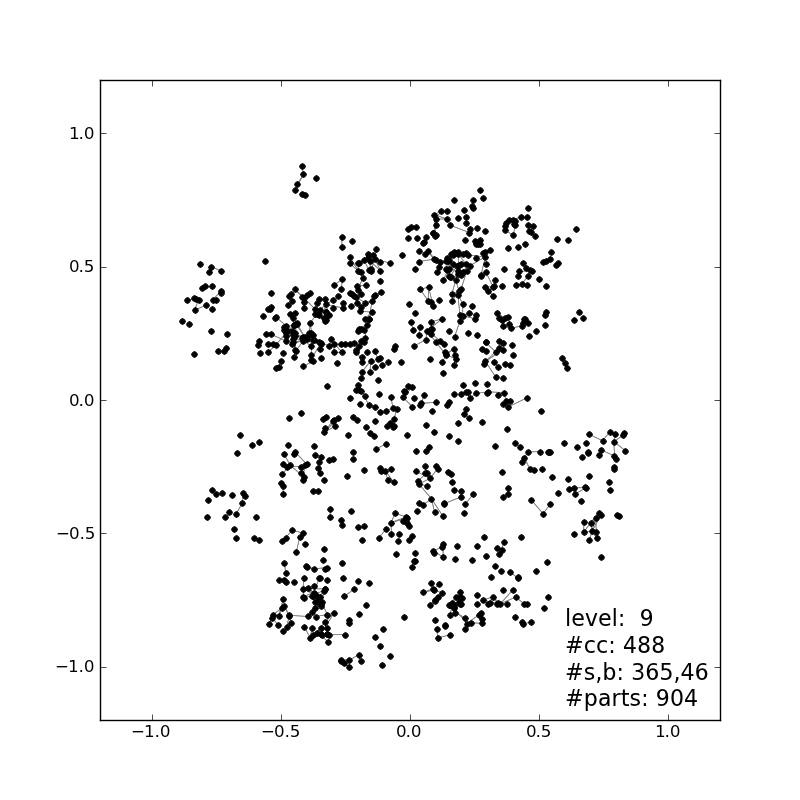
\includegraphics[scale=0.3,bb = 0 0 200 100, draft, type=eps]{/Users/jj374/castle/5hs-paper2/cc_paper-svn/1_cc_illustration/cc-2.3-009.png}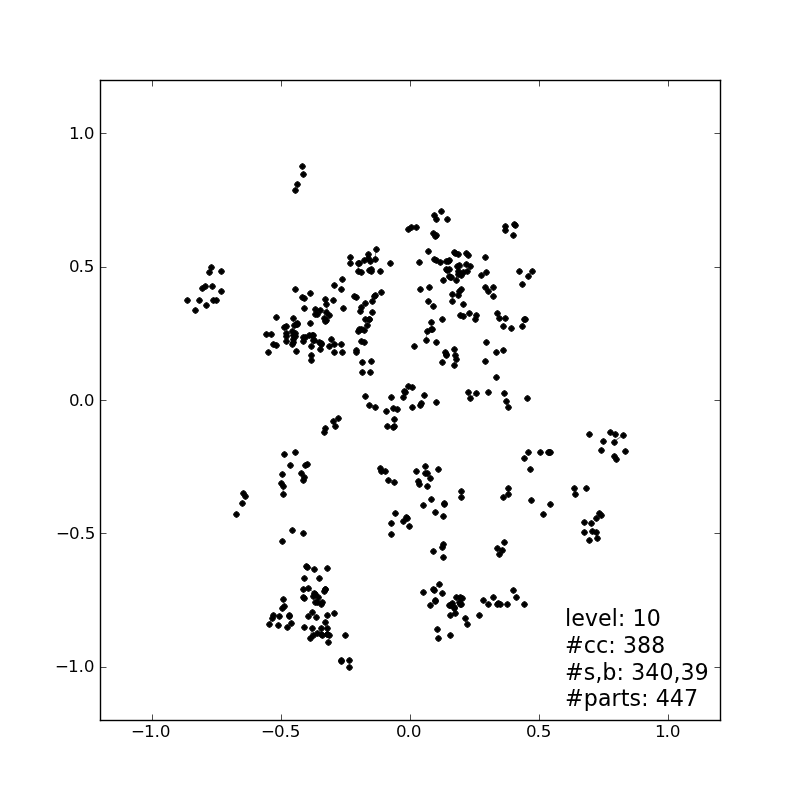
\includegraphics[scale=0.3,bb = 0 0 200 100, draft, type=eps]{/Users/jj374/castle/5hs-paper2/cc_paper-svn/1_cc_illustration/cc-2.3-010.png}

\caption{\label{fig:time-step-graph} Time step graph generated by $\tau(i,j)$
for fractal initial conditions for four consecutivelly decreasing
pivot time step values $h$.}
\end{figure}


Figure \ref{fig:time-step-graph} visualises the time step graph for
a system of fractal initial conditions for a series of consecutivelly
decreasing values of the pivot time step $h$. As the pivot time step
$h$ decreases, the set of interactions (and associated particles)
that \emph{cannot} be evaluated at the current pivot time step gradually
reduces. Note that although for visualisation purposes, we plot the
time step graph of the entire system for varying $h$, the CC splitting
method we are about to introduce generally calculates the decomposition
for the entire system only once, at the lowest time step. At higher
time steps, the connected components search is only performed for
parts of the system. The intuition behind using this kind of a decomposition,
something which we also consider an awesome example of interdisciplinary
exchange of ideas, comes from the principle of clustering via maximizing
the margin between individual clusters.\cite{Duan:2009kh}

We use the following notation to describe the partitioning of the
particles resulting from the connected component search. The sets
$C_{i},\, i=1\ldots K$ contain vertices of $K$ non-trivial connected
components. The set $R$ (``rest set'') contains all particles in
trivial connected components.%
\footnote{A \emph{trivial connected component} is a connected component with
exactly one vertex and a \emph{non-trivial connected component} is
a connected component with at least two vertices.%
} Based on the particle sets $C_{i}$ and $R$, we decompose the Hamiltonian
of the system into following terms

\[
H\rightarrow H_{C}+H_{R}+V_{CC}+V_{CR}
\]
which are defined as follows.
\begin{eqnarray*}
H_{C} & = & \underset{i=1}{\overset{K}{\sum}}H_{C_{i}}=\underset{i=1}{\overset{K}{\sum}}\left(\underset{j\in C_{i}}{\overset{}{\sum}}T_{j}+\underset{\substack{j,k\in C_{i}\\
i<j
}
}{\overset{}{\sum}}V_{jk}\right)\\
H_{R} & = & T_{R}+V_{R}=\underset{i\in R}{\overset{}{\sum}}T_{i}+\underset{\substack{i,j\in R\\
i<j
}
}{\overset{}{\sum}}V_{ij}\\
V_{CC} & = & \underset{\substack{i,j=1\\
i<j
}
}{\overset{K}{\sum}}V_{C_{i}C_{j}}=\underset{\substack{i,j=1\\
i<j
}
}{\overset{K}{\sum}}\left(\underset{\substack{k\in C_{i}\\
l\in C_{j}
}
}{\overset{}{\sum}}V_{kl}\right)\\
V_{CR} & = & \underset{i=1}{\overset{K}{\sum}}V_{C_{i}R}=\underset{i=1}{\overset{K}{\sum}}\left(\underset{\substack{j\in C_{i}\\
k\in R
}
}{\overset{}{\sum}}V_{jk}\right)
\end{eqnarray*}
The term $H_{C}$ consists of individual closed Hamiltonians $H_{C_{i}}$
obtained from the connected component search. By the definition of
a connected component, all drifts and some of the kicks cannot be
evolved at the time step $h$ without violating the time step criteria.

The term $H_{R}$ consists of the closed Hamiltonian formed by all
of the particles in the rest system. All of the drifts and kicks in
this system can be evolved at the current time step $h$. 

The term $V_{CC}$ contains all kicks between particles that are in
\emph{different} connected components. These kicks can be evolved
at the time step $h$.

We explicitly point out that $V_{CC}$ contains slow interaction terms
between connected components that can be evolved at the current time
step. In other words, the CC-split isolates into $V_{CC}$ the terms
that are evolved inefficiently in the HOLD method as discussed previously.

Having defined a decomposition of the Hamiltonian using connected
components, we perform a split of the system by evolving connected
components $H_{C}$ at a higher time step and everything else at the
current time step.

\begin{eqnarray*}
\operatorname{E}_{h,H} & = & \operatorname{E}_{h,H\rightarrow H_{C}+H_{R}+V_{CC}+V_{CR}}\\
 & \approx & \operatorname{E}_{h/2,H_{C}}\,\operatorname{E}_{h,H_{R}+V_{CC}+V_{CR}}\operatorname{E}_{h/2,H_{C}}
\end{eqnarray*}
The (independent) Hamiltonians of the connected components are evolved
separately at a higher time step $h/2$ by recursively applying the
same connected component split operator.

\[
\operatorname{E}_{h/2,H_{C}}=\overset{K}{\underset{i=1}{\prod}}\operatorname{E}_{h/2,H_{C_{i}}}
\]
Everything else can be evaluated at the time step $h$. We apply a
second order split and obtain the following explicit formula for calculating
the time evolution.
\begin{eqnarray*}
\operatorname{E}_{h,H_{R}+V_{CC}+V_{CR}} & = & \operatorname{E}_{h,T_{R}+V_{R}+V_{CC}+V_{CR}}\\
 & \approx & \operatorname{D}_{h/2,T_{R}}\operatorname{K}_{h,V_{R}+V_{CC}+V_{CR}}\operatorname{D}_{h/2,T_{R}}\\
 & = & \operatorname{D}_{h/2,T_{R}}\operatorname{K}_{h,V_{R}}\operatorname{K}_{h,V_{CC}}\operatorname{K}_{h,V_{CR}}\operatorname{D}_{h/2,T_{R}}
\end{eqnarray*}



\subsection{Implementation}

Our implementation of the CC split is in the file \texttt{evolve\_split\_cc.c}
of the HUAYNO integrator. The implementation aims to use existing
code as much as possible. The \texttt{sys} data structure is extended
with a \texttt{sys}-type pointer \texttt{next\_cc} to be usable as
a singly linked list for storing the connected components.

The connected component algorithm is implemented as a breadth-first
search in the function \texttt{split\_cc} and reshuffles an underlying
array containing the particles, just like the implementation of the
HOLD split. The only dynamic memory allocation performed by the routine
is for new \texttt{sys} structures to store the pointers to the end
points of the connected components.

Explicit sanity checks of the connected components algorithm can be
turned on by with the macro \texttt{CC2\_SPLIT\_CONSISTENCY\_CHECKS}
macro (they are turned off by default due to performance reasons).


\section{Tests}

\begin{figure}[p]
\begin{centering}
%\includegraphics[scale=0.4]{4_nitadori2008}
\par\end{centering}

\caption{\label{fig:plummer-unsoftened}Time evolution of the conserved quantities:
total energy $E$ (top left), linear momentum $\mathbf{p}$ (top right),
center of mass velocity $\mathbf{v}_{cm}$ (bottom left) and angular
momentum $\mathbf{L}$ (bottom right) for the $1024$ body Plummer
sphere.\protect \\
Time evolution of the Lagrangian radii (left graph, dashed lines,
from top to bottom 90\%, 50\%, 10\% and 1\%), core radius (left graph,
solid lines) and core density (right graph) for the $1024$ body Plummer
sphere integration.\protect \\
Performance metrics: calculation time (top left), time step evaluation
count (top right), kick evaluation count (bottom left) and drift evaluation
count (bottom right) for the $1024$ body Plummer sphere.\protect \\
TODO: \protect \\
(1) fix the overflow bug in EXTRAPOLATE kick+time step evaluations\protect \\
(2) remove the background grid (from all plots)}
\end{figure}


We integrate an equal-mass $1024$-body Plummer sphere under a softening
($\varepsilon=1/256$) for $700$ $N$-body time units using an accuracy
parameter of $\eta=0.01$. The setup is chosen to match the long-term
integration tests in \cite[their section 3.2]{Nitadori:2008gt}.

On Figure \ref{fig:plummer-unsoftened}, we visualise the error in
conserved quantities (top four plots), behaviour of the solution (middle
two plots), and the performance metrics (bottom four plots). We compare
our novel CC splitting method with the HOLD method introduced in \cite{Pelupessy:2012if},
as well as reference implementation of a conventional block time stepping
scheme that extrapolates the positions of particles in lower time
step bins when calculating the movement of particles in faster time
step bins (EXTRAPOLATE).

While all three methods show similar energy conservation properties,
only HOLD and CC maintain centre of mass, linear momentum and angular
momentum near machine precision. As noted previously, this is caused
by unsynchronized kicks which are only present in the EXTRAPOLATE
scheme.\cite{Pelupessy:2012if} 

The solutions obtained by all three methods behave as expected in
terms of Lagraingian radii, the core radius and the core density,
reproducing known previous results.

Looking at the performance metrics, both HOLD and CC show a significant
reduction in the number of kick, drift and time step evaluations compared
to EXTRAPOLATE. This is reflected in the drastic reduction in CPU
time used.

Compared to the HOLD method, the CC method uses roughly 25\% less
kick evaluations, and 50\% less time step evaluations. As the Plummer
sphere is a spherically symmetric problem (and we are using softening),
we would not expect the CC split to have a significant advantage over
the HOLD method in terms of the number of kick evaluations, so the
magnitude of the decreases observed is somewhat unexpected.

\begin{figure}[p]
\begin{centering}
%\includegraphics[scale=0.4]{5_kokkotas2010/conservation-plummer_cons00}
\par\end{centering}

\begin{centering}
%\includegraphics[scale=0.4]{5_kokkotas2010/dynamics-plummer_cons00}
\par\end{centering}

\begin{centering}
%\includegraphics[scale=0.4]{5_kokkotas2010/kokkotas2010_cputime}
\par\end{centering}

\caption{\label{fig:plummer-core-collapse} A comparison of three splitting
methods on a $1024$-body Plummer sphere through core collapse in
terms of conservation (top 4), behaviour of the solution (next two)
and computation time (bottom).}
\end{figure}


Next, we evolve an equal-mass $1024$-body Plummer sphere without
softening through core collapse. This setup is chosen to match a test
used on a modern implementation of a fourth-order Hermite scheme with
block time steps.\cite[their section 3.4.1]{Konstantinidis:2010hx}

Figure \ref{fig:plummer-core-collapse} visualises the error in conserved
quantities, the behaviour of the solutions, and performance metrics
for HOLD, CC and a modification of the CC split with a dedicated Kepler
solver (CC\_KEPLER) that is used for evolving connected components
consisting of two particles (the implementation of the Kepler solver
is based on \cite{bate1971fundamentals}). For all three methods,
the solutions are realistic in terms Lagrangian radii, core radius
and core density, with core collapse at roughly $350$$N$-body time
units. Energy conservation is comparable with what is observed in
\cite{Konstantinidis:2010hx}, with linear momentum conserved around
machine precision. While the incorporation of a dedicated Kepler solver
has a small but notable negative effect on angular momentum conservation,
computation time at and after core collapse is drastically reduced
compared to the HOLD and CC methods. 

\begin{figure}[p]
\begin{centering}
%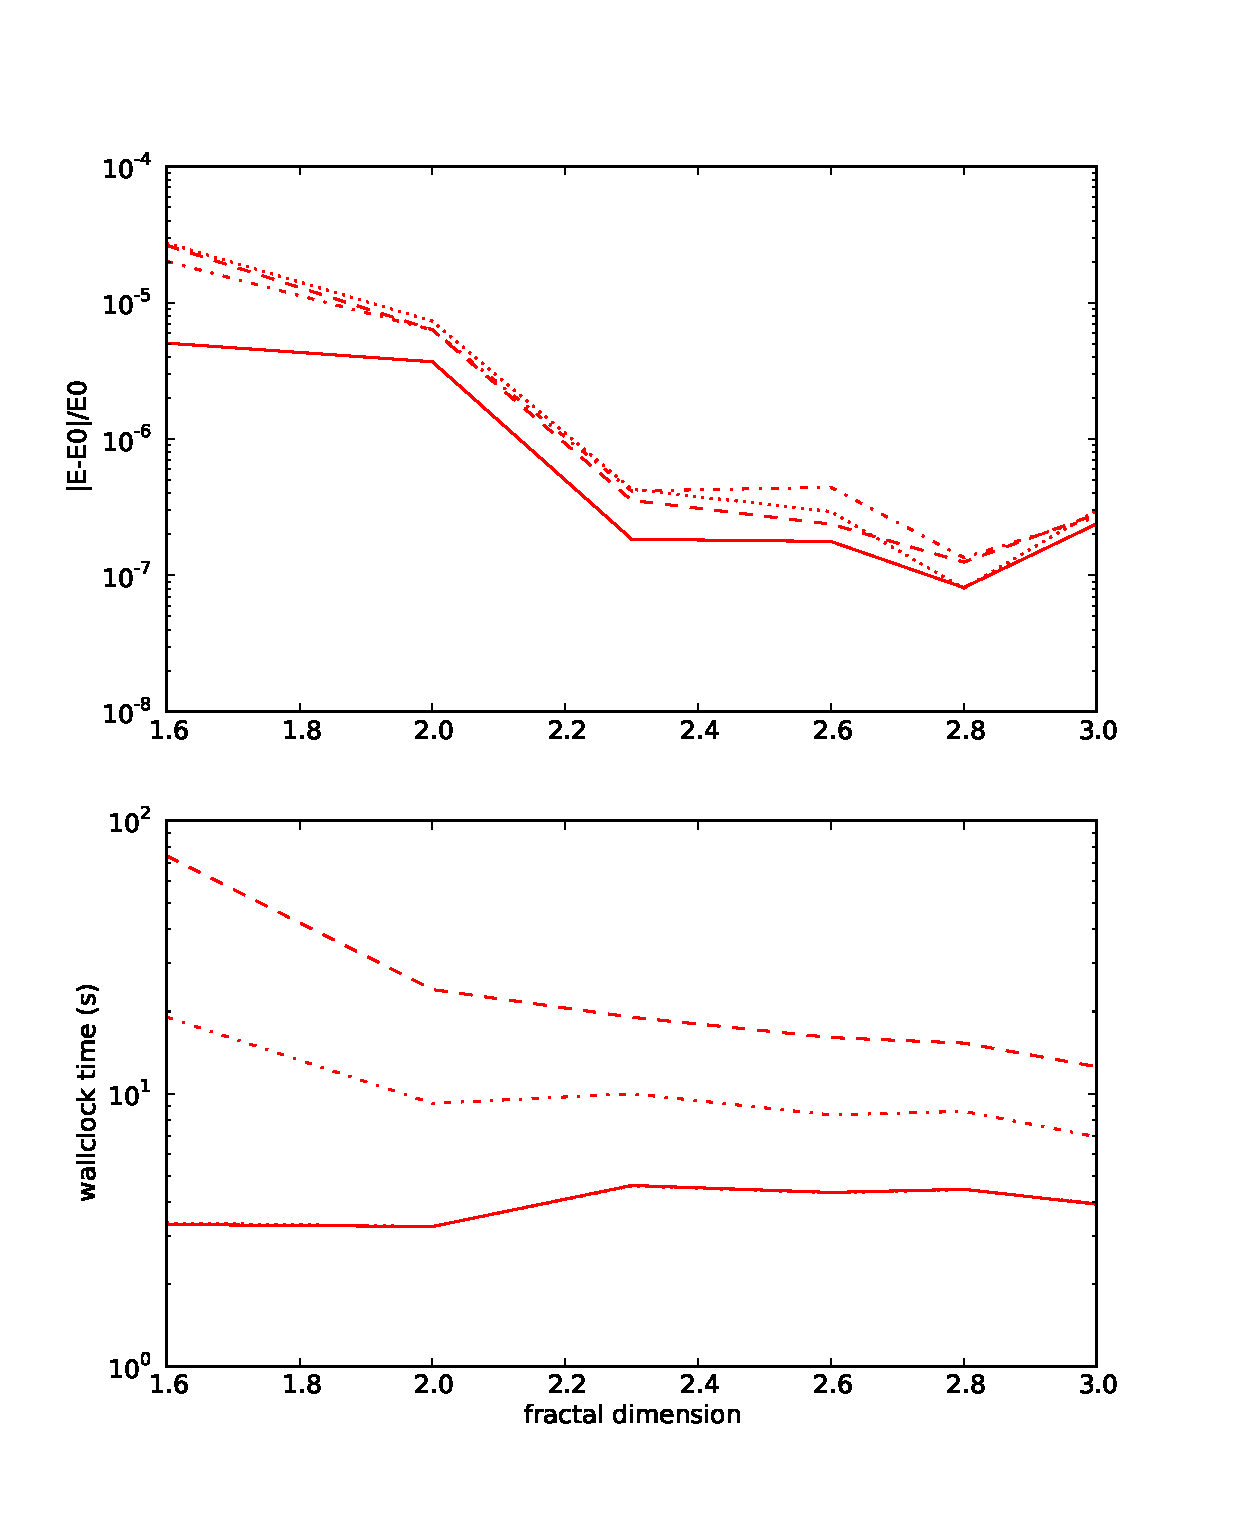
\includegraphics[scale=0.4]{6_fractal/fractal_dimension_dE_time}
\par\end{centering}

\caption{\label{fig:fractal-initial-conditions}Energy error and runtime as
a function of fractal dimension for different integrators. Plotted
are the energy error (top panel) and runtime (bottom panel) of runs
with 1024 particles as a function of the fractal dimension of the
particle distribution for the EXTRAPOLATE (dashed line), SF-split
(dash-dotted line) and the CC (dotted) and CC\_KEPLER (drawn) split
integrators. Note that all integrators have similar error behaviour,
while the run time increases for decreasing fractal dimension (so
for more structured particle distributions) for the EXTRAPOLATE and
SF split integrators, while the runtime is flat and even decreases
slightly for lower fractal dimension for the CC integrators. }
\end{figure}


We proceed by integrating a set of fractal initial conditions that
model the distribution of stars in a ``pre-Plummer sphere'' stage.{[}Goodwin?
/FIXME/{]} These initial conditions are parametrized by a fractal
dimension that characterises the ``sparseness'' of the system. We
use $\eta=0.03$, and integrate a system of $N=1000???$ particles
under an unsoftened potential(???) for $0.25$$N$-body units. 

Figure \ref{fig:fractal-initial-conditions} plots energy conservation
and wallclock time at the end of the simulation, averaged over 10
runs, as a function of the fractal dimension. Consistently across
all fractal dimension values, CC and CC\_KEPLER are the fastest, followed
by HOLD and EXTRAPOLATE. The differences in the efficiencies are bigger
for smaller fractal dimensions (where the system is more ``sparse''),
and smaller for larger fractal dimensions. For a fractal dimension
of $3$, the initial conditions (and results) are similar to an ordinary
Plummer sphere.

\begin{figure}[p]
\begin{centering}
Here be dragons.
\par\end{centering}

\caption{\label{fig:plummer-of-binaries-scaling}Scaling of the Plummer sphere
with binaries problem.}
\end{figure}


As a final test, we take an $1024$-body Plummer sphere and replace
$X\%$ of the stars with a binary system with semimajor axis $a$.
We use an unsoftened potential and evolve the system for $Y$$N$-body
time.

Figure \ref{fig:plummer-of-binaries-scaling} visualises the energy
conservation and wall-clock time as a for varying values of the semimajor
axis $a$. For large $a$, the introduced binaries are generally unbounded,
and the results are equivalent to evolving an ordinary Plummer sphere.
As $a$ decreases, the introduced binaries become bounded and their
interactions start dominating in the integration time, leading to
a significant advantage for CC and CC\_KEPLER methods.

\section{Discussion}

We have constructed a novel method for direct integration of $N$-body
systems based on the decomposition of the Hamiltonian guided by the
connected components of the time step graph. We have shown that in
comparison to existing splitting methods, notably the HOLD split,
the CC split is particularly effective for integrating multi-scale
problems. Further, we have not encountered a situation where the HOLD
method would be the preferred over the CC split.

We have already demonstrated that the partitioning used in the CC
split has additional uses beyond reducing the number of kicks and
time steps compared to the HOLD split by integrating special treatment
of close binaries into the CC integrator. We achieved this by adding
a single Kepler solver call for the condition where the successive
partitioning leads to a connected component with two particles. There
is no need for an explicit search for potential close encounters,
neighbour lists, or the addition of free parameters, such as distance
thresholds, that would need manual tuning.\cite{Konstantinidis:2010hx}
This also suggests a straightforward approach to a more accurate treatment
of many-body close encounters by using a higher order solver to evolve
connected components below a certain number of particles and/or above
a specific pivot time step $h$.

/TODO: Parallelisation: (1) shared memory: evolve components in parallel
(not obvious when to start a new thread; (2) GPU: kicks/time steps
would have to be evaluated in larger blocks (several components at
the same time?); (3) graph algorithms on GPUs are an open area of
research/

Further, it could be conceivable to speed up the evaluation of long-range
interactions between different connected components ($V_{CC}$ in
the CC decomposition formula) through a centre-of-mass (or multipole)
approximation that form the basis of tree codes.\cite{Barnes:1986ed}
As long-range interactions between two connected components are evaluated
symmetrically, this leaves open the possibility of obtaining most
of the speedup possible through the use of a tree code while still
maintaining linear and angular momentum conservation near machine
precision. A potential pitfall with this approach could arise from
the fact the time step criterion $\tau(i,j)$ used in constructing
the connected components is only partially determined by the coordinates
of the particles. As such, particles in the same connected component
may occupy an ``non-compact'' region in physical space, making multipole
approximation difficult.

Additional performance gain could also be obtained by changing the
splitting of the Hamiltonian to obtain a partitioning that is closer
to the formal criteria discussed in the Methods section. For example,
a variation of the HOLD method where the partitioning step is done
on the list of interactions (instead of particles) leads to a splitting
that is formally optimal: every \emph{interaction} in the system is
evaluated at the closest time step in the power of two hierarchy.
An implementation of this method is available in the current HUAYNO
code under the name OK-split (OK stands for Optimal Kick). At present,
the performance of this integrator is not competitive compared to
the CC-split. For example, in the $1024$-body smoothed Plummer sphere
test, the OK method gives a reasonable solution that is comparable
to the HOLD and CC methods in terms of momenta conservation and the
dynamics of the radii while using significantly fewer kicks and time
step evaluations. However, the OK method does show significantly worse
energy conservation (around $10^{-2}$ at the end of the test, compared
to $10^{-5}$ for HOLD and CC). It is however worth pointing out that
while the possibility of direct $N$-body integration with \emph{interaction-based
time steps} has been previously considered in \cite[sec 4.2]{Nitadori:2008gt},
the OK-split is the first workable implementation of this idea that
we are aware of.

One possible reason for the decline in energy conservation in our
implementation of the OK-split is the use of the explicit but approximate
time step criteria introduced in \cite{Pelupessy:2012if}. Notably,
the criteria only depends on the state of the two interacting particles.
This leads to an underestimate of the time step for interactions with
a large concentration of mass along the ``line of sight'' between
the two particles. One example where this underestimation could play
a significant role is an interaction between any two particles at
the opposite edges of a Plummer sphere. Note how this situation is
handled differently in the CC-split where the time step of an interaction
is essentially determined by the largest connected component that
still includes both particles.

Our implementations of the new integration methods are incorporated
in the HUAYNO integration code and are made freely available as a
part of the AMUSE framework. 


\section{Acknowledgements}

This work was supported by the Netherlands Research Council NWO (Grants
XX/YY/ZZ) and by the Netherlands Research School for Astronomy (NOVA).
J\"urgen J\"anes acknowledges support from the Archimedes
Foundation, Estonian Students' Fund USA, Estonian Information Technology
Foundation and Skype.

\bibliographystyle{apalike}
\bibliography{cc_paper}

\end{document}
